% !TeX root = ../thuthesis-example.tex

\chapter{模型的构建与优化}

\section{数据来源与免疫相关标签体系构建}
蛋白质必需性具有显著的层级差异性与情境依赖性。在此基础上，本研究重新组织数据来源，并构建“基础生存约束 + 免疫情境功能依赖”双标签体系。
\subsection{人类遗传约束数据}
为刻画蛋白质在人类种群尺度上的基础功能重要性，本研究引入人类基因组聚合数据库（Genome Aggregation Database, gnomAD）v4.1 提供的基因层面遗传约束指标基因功能缺失观察值/期望值比例置信上界（Loss-of-function Observed/Expected Upper bound Fraction, LOEUF）\cite{karczewski2020mutational}。该指标建立在大规模外显子测序数据对功能缺失变异（loss-of-function, LoF）进行统计建模的框架之上，其理论基础来源于外显子组聚合联盟（Exome Aggregation Consortium, ExAC）项目对 60,706 例人类外显子数据的系统分析 \cite{lek2016protein}。该研究通过构建突变率驱动的中性模型，对每个基因在无选择压力假设下的 LoF 变异期望数量进行估计，从而为定量评估基因所受负选择约束程度提供了统计基准。

对于任一基因 $g$，设其观测到的 LoF 变异数量为 $O_g$，在中性突变模型下的期望 LoF 变异数量为 $E_g$，则有
\begin{equation}
    E_g = \sum_{i \in g} \mu_i \cdot C_i,    
\end{equation}
其中 $\mu_i$ 表示在特定三核苷酸序列背景下第 $i$ 个位点的突变率，$C_i$ 表示覆盖度与检测概率校正项。由此可定义观测/期望比值（observed/expected, O/E）
\begin{equation}
    R_g = \frac{O_g}{E_g}.
\end{equation}
当 $R_g \ll 1$ 时，说明该基因中的 LoF 变异显著少于期望值，提示其在种群层面受到强负选择压力。为提高估计的稳健性，gnomAD 对 $R_g$ 构建置信区间，并将其 $90\%$ 置信区间上界定义为 LOEUF，即
\begin{equation}
    \mathrm{LOEUF}_g = U_{0.90}(R_g),
\end{equation}
其中 $U_{0.90}(\cdot)$ 表示 $R_g$ 的 $90\%$ 置信上界。由于采用上界估计，该指标在统计上具有保守性：即便观测变异数较少，也不会过度夸大基因的不耐受程度。因此，$\mathrm{LOEUF}_g$ 越小代表基因对功能缺失越不耐受，进化约束越强。

从生物学意义上看，LOEUF 反映的是基因在长期进化过程中所承受的群体选择压力，可近似理解为种群尺度的功能必要性或剂量敏感性信号。然而，该指标并不区分组织或细胞类型，其估计结果更接近跨组织平均选择效应。因此，本研究将 LOEUF 用作 Human-level 必需性的监督来源，而不将其视为特定中性粒细胞激活状态的直接表征。

在具体标签构建过程中，我们以 $\mathrm{LOEUF}=0.6$ 作为区分阈值，定义
\begin{equation}
    y_g=
    \begin{cases}
    1, & \mathrm{LOEUF}_g \le 0.6,\\
    0, & \mathrm{LOEUF}_g > 0.6,
    \end{cases}
\end{equation}
其中 $y_g=1$ 表示种群层面功能不耐受（Human-level essential），$y_g=0$ 表示相对耐受。通过基因到蛋白的映射，将上述标签转化为蛋白层面的监督信号，最终构建 15,234 个必需蛋白标签与 53,642 个非必需蛋白标签。

基于上述数据，我们训练 Human-level 模型学习从蛋白序列 $\mathbf{s}$ 到种群层面必需性概率的映射：
\begin{equation}
    PES_{\mathrm{human}}(\mathbf{s}) = \Pr(y=1 \mid \mathbf{s}; \theta),
\end{equation}
其中 $\theta$ 表示模型参数，$PES_{\mathrm{human}}$ 定义为 Human-level Protein Essentiality Score。该评分反映蛋白序列所对应的进化约束强度，为后续与 Immune-level 模型输出进行比较奠定基准。Human-level 表示蛋白在人群进化约束层面的基础生存依赖。通过在统一序列空间中建立种群尺度的必需性表征，本研究进一步引入免疫相关细胞系 CRISPR 依赖数据进行情境适配，从而实现从一般必需性到免疫情境相关依赖性的层级建模。

\subsection{免疫细胞系必需性数据}

为刻画蛋白质在免疫情境中的功能依赖性，本研究引入 Project Score 数据库提供的基因必需性数据。该数据库来源于 Nature 2019 年报道的全基因组 CRISPR--Cas9 敲除筛选研究 \cite{behan2019prioritization}。在该研究中，研究者通过包含数万个 sgRNA 的文库对数百个人类细胞系进行系统性基因敲除，并基于 sgRNA 丰度变化评估基因对细胞适应度（cellular fitness）的影响。

在实验原理层面，设第 $c$ 个细胞系中第 $g$ 个基因对应 sgRNA 在敲除前后的丰度分别为 $A_{g,c}^{(0)}$ 与 $A_{g,c}^{(t)}$，则其对数丰度变化可表示为
\begin{equation}
    \Delta_{g,c} = \log_2 \left( \frac{A_{g,c}^{(t)}}{A_{g,c}^{(0)}} \right).
\end{equation}

当基因敲除显著降低细胞增殖能力时，其对应 sgRNA 在群体中的比例将逐渐减少，从而表现为显著负的丰度变化。基于此原理，研究者进一步构建经 copy-number 校正与批次效应校正后的基因依赖评分，用以量化基因对特定细胞系存活的依赖强度。

在数据库发布阶段，Project Score 数据库在连续依赖评分基础上提供了二值化的必需性标签矩阵。该矩阵可形式化表示为
\begin{equation}
    y_{g,c} \in \{0,1\},
\end{equation}
其中 $y_{g,c}=1$ 表示基因 $g$ 在细胞系 $c$ 中被判定为必需基因，$y_{g,c}=0$ 表示非必需基因。该二值矩阵已在 PIC 模型中作为细胞层面必需性监督数据使用 \cite{kang2024comprehensive}。

在本研究中，为聚焦免疫情境相关依赖信号，我们从 Project Score 全部细胞系集合 $\mathcal{C}_{all}$ 中筛选出 14 个具有免疫来源或免疫相关表型特征的细胞系，构建免疫子集 $\mathcal{C}_{immune}$。这些细胞系虽然并不直接等同于原代中性粒细胞，但其依赖谱能够提供与免疫效应执行相关的高应激功能信号，尤其对应氧化应激、膜运输与膜重塑活跃以及颗粒/溶酶体负荷升高等过程，因此可作为构建 Immune-level 监督标签的观测基础。对于任一基因 $g$，定义其在免疫子集中的必需性比例为
\begin{equation}
    \bar{y}_g^{immune}
    =
    \frac{1}{|\mathcal{C}_{immune}|}
    \sum_{c \in \mathcal{C}_{immune}}
    y_{g,c}.
\end{equation}

该比例反映基因在免疫情境相关高应激功能背景下被判定为必需的频率。为构建 Immune-level 监督标签，我们定义
\begin{equation}
    z_g=
    \begin{cases}
    1, & \bar{y}_g^{immune} \ge 0.8,\\
    0, & \text{otherwise},
    \end{cases}
\end{equation}
$z_g=1$ 表示该基因在该高应激功能情境相关细胞集合中表现为一致性依赖基因。

需要强调的是，尽管 Project Score 数据覆盖 300 余个不同来源的细胞系 \cite{behan2019prioritization}，本研究并未直接纳入全部细胞系进行训练，而是基于研究目标限定细胞谱系空间，仅保留免疫相关子集。在条件概率意义下，本研究建模的是
\begin{equation}
    P(z=1 \mid \mathbf{s}, \text{immune-stress context}),
\end{equation}
而非无条件概率 $P(z=1 \mid \mathbf{s})$。该策略能够降低跨谱系异质性带来的噪声干扰，提高模型对免疫情境相关依赖信号的分辨能力。Immune-level 表示蛋白在免疫效应执行相关高应激功能情境中的条件性依赖。本文所称免疫情境，是指免疫效应执行过程中由氧化应激增强、胞内运输与膜重塑活跃以及颗粒/溶酶体功能负荷升高共同构成的高应激功能情境。鉴于本文始终以中性粒细胞为研究对象，该情境在生物学解释和实验验证层面进一步具体化为急性炎症应答中以氧化爆发增强和颗粒/溶酶体功能负荷升高为特征的活化中性粒细胞状态。由此，Human-level 与 Immune-level 的比较可理解为基础生存依赖与条件性依赖的层级比较，而中性粒细胞则是本文进行生物学聚焦与后续验证的具体研究对象。

基于上述免疫必需性标签，我们训练 Immune-level 模型学习蛋白序列 $\mathbf{s}$ 与免疫情境相关依赖性之间的映射关系：
\begin{equation}
    PES_{\mathrm{immune}}(\mathbf{s})
    =
    \Pr(z=1 \mid \mathbf{s}; \phi),
\end{equation}
其中 $\phi$ 表示模型参数。通过与 Human-level 模型输出进行比较，可进一步定义
\begin{equation}
    \Delta PES(\mathbf{s})
    =
    PES_{\mathrm{immune}}(\mathbf{s})
    -
    PES_{\mathrm{human}}(\mathbf{s}),
    \label{eq:delta_pes}
\end{equation}
用于识别在种群层面并非高度受限，但在免疫情境中表现出显著依赖的候选蛋白。

\subsection{蛋白质序列获取与标准化处理}

在监督标签层面，无论是基于 LOEUF 的人群层面功能不耐受信息，还是基于 Project Score 的细胞依赖信息，原始数据均以基因为基本单位。然而，本研究的模型输入为蛋白质氨基酸序列，因此需要在建模前完成从“基因层面标签”到“蛋白层面序列”的标准化映射。

首先，根据Ensembl Gene ID，将基因映射至 UniProt 数据库（UniProtKB/Swiss-Prot）对应条目 \cite{consortium2023uniprot}。使用Ensembl BioMart API编写脚本从 BioMart 中直接获取蛋白质序列。为避免不同转录本导致的序列歧义问题，本研究遵循 PIC 框架 \cite{kang2024comprehensive}，仅保留每个基因对应的 canonical isoform 作为代表序列。若某基因存在多个蛋白条目，则优先选择经过人工注释且标记为“Reviewed”的 Swiss-Prot 条目；对于无法匹配至唯一蛋白序列的基因，则予以剔除。

在获得蛋白序列后，进一步进行如下预处理步骤：  
（1）去除含有非标准氨基酸字符（如 B、Z、J、U、O）的序列；  
（2）过滤极短序列（长度 < 30 aa），以避免噪声蛋白或片段序列对模型训练造成干扰；  
（3）对重复序列进行去重，确保同一氨基酸序列不会在训练集中重复出现；  
（4）对长度超过预设上限的序列进行截断或分段处理，以满足预训练 PLM（ProtT5）的最大输入长度限制。

最终获得用于建模的蛋白序列集合 $\{s_i\}$，
并将基因层面的监督标签精确映射至对应的蛋白序列层面。
同时，为保证样本的可追溯性与跨数据库一致性，每条序列均保留其唯一蛋白标识符（Protein ID）。

因此，构建的训练数据集可形式化表示为
\begin{equation}
\mathcal{D} = \{(p_i, s_i, y_i)\}_{i=1}^{N},
\end{equation}
其中 $p_i$ 表示第 $i$ 个蛋白的唯一标识符（如 UniProt ID），$s_i$ 表示对应蛋白的氨基酸序列，$y_i$ 表示其必需性监督标签，$N$ 为最终纳入建模的蛋白样本总数。监督标签 $y_i$ 为二分类变量，1 表示必需蛋白，0 表示非必需蛋白。

根据预测层级的不同，进一步构建两个层级特异性数据集：
\begin{equation}
\mathcal{D}^{(H)} = \{(p_i, s_i, y_i^{(H)})\}_{i=1}^{N_H}, \qquad
\mathcal{D}^{(I)} = \{(p_i, s_i, y_i^{(I)})\}_{i=1}^{N_I},
\end{equation}
其中 $y_i^{(H)}$ 表示 Human-level 必需性标签，$y_i^{(I)}$ 表示 Immune-level 必需性标签，$N_H$ 与 $N_I$ 分别表示对应层级的数据规模。

由于蛋白质必需性最终体现为蛋白分子功能缺失对细胞适应度或个体存活能力的影响，
因此将基因层级标签信息映射至蛋白序列层级具有明确的生物学合理性。

\section{模型架构设计}
\subsection{序列嵌入模块：ProtT5 表示学习机制}

为从蛋白质氨基酸序列中提取具有结构与功能语义的信息，本研究采用基于 Transformer 架构的蛋白语言模型 ProtT5 作为序列嵌入层。ProtT5 属于 ProtTrans 框架中的预训练模型，通过在大规模未标注蛋白质数据库上进行自监督学习，构建通用的蛋白序列表示空间。

ProtT5 基于 T5（Text-to-Text Transfer Transformer）架构构建，其核心为多层 Transformer 结构。Transformer 通过自注意力（Self-Attention）机制在单层内建立序列中任意两个位置之间的依赖关系，从而实现全局上下文建模。相比基于递归或卷积的序列模型，该结构能够有效捕捉远距离残基之间的协同关系，这对于蛋白质功能建模尤为重要，因为催化位点、结构域耦合或功能调控区域往往分布于序列的不同位置。在本研究中，主要使用 ProtT5 编码器部分输出残基级嵌入表示。

ProtT5 的训练采用自监督掩码语言建模（Masked Language Modeling, MLM）任务。设蛋白质序列为：

\begin{equation}
S = (a_1, a_2, \dots, a_L)
\end{equation}

在预训练阶段，随机选择一部分位置集合 $M \subset \{1, \dots, L\}$ 进行遮蔽。模型的训练目标是预测被遮蔽位置的真实氨基酸类型，其损失函数定义为：

\begin{equation}
\mathcal{L}_{MLM}
=
- \sum_{i \in M}
\log P_\theta(a_i \mid S_{\setminus M})
\end{equation}

其中：

\begin{itemize}
    \item $\mathcal{L}_{MLM}$ 为掩码语言建模损失；
    \item $M$ 为被遮蔽位置集合；
    \item $a_i$ 为第 $i$ 个位置的真实氨基酸；
    \item $S_{\setminus M}$ 表示将集合 $M$ 中位置替换为 \texttt{<mask>} 后的输入序列；
    \item $P_\theta(a_i \mid S_{\setminus M})$ 为模型在参数 $\theta$ 下对该位置残基的预测概率；
    \item 负号表示最小化负对数似然，即等价于最大化正确残基的对数概率。
\end{itemize}

该训练目标迫使模型利用上下文信息恢复缺失残基。由于蛋白质序列在进化过程中受到结构稳定性、功能活性及选择压力的约束，残基之间存在复杂统计依赖关系，因此最小化上述损失的过程，本质上是在逼近蛋白质的进化统计分布。模型通过学习“在给定上下文条件下哪种氨基酸更可能出现”，隐式捕捉了残基共现模式与进化保守性信号。

经过预训练后，ProtT5 将离散氨基酸序列映射为残基级嵌入矩阵：

\begin{equation}
\mathbf{H} = f_\theta(S) \in \mathbb{R}^{L \times d}
\end{equation}

其中 $\mathbf{h}_i \in \mathbb{R}^{d}$ 表示第 $i$ 个残基在全局语境下的上下文嵌入表示。

已有研究表明，该嵌入空间能够通过简单线性映射预测二级结构、溶剂可及性以及功能域类别，说明其隐藏表示中已编码与蛋白质结构和功能相关的统计特征\cite{elnaggar2022prottrans}。因此，该表示不仅包含序列级信息，还隐式包含结构约束与进化选择压力的痕迹。

蛋白质必需性通常与功能域完整性、关键催化位点保守性及结构稳定性密切相关，这些因素在进化过程中具有显著保守性，并体现在残基共现统计模式中。因此，可将必需性预测表示为：

\begin{equation}
\hat{y} = g_\phi(f_\theta(S))
\end{equation}

其中 $f_\theta(S)$ 为 ProtT5 嵌入表示，$g_\phi$ 为后续判别网络。

由于嵌入空间中已编码与结构和功能相关的统计信息，必需与非必需蛋白在该连续语义空间中往往具有不同分布特征，从而使必需与非必需蛋白在嵌入空间中呈现可区分的分布特征。

\begin{figure}[!htbp]
    \centering
    \includegraphics[width=1\linewidth]{figures/protT5.png} 
    \caption[ProtT5 原理示意图]{ProtT5 原理示意图。该图展示了预训练蛋白语言模型从氨基酸序列输入、上下文表征学习到下游任务迁移的基本框架，说明序列嵌入如何作为后续必需性判别模块的统一表示基础。}
    \label{fig:prott5_schematic}
\end{figure}

\subsection{分类模块}

在获得预训练 PLM 输出的残基级上下文嵌入表示后，仅依赖原始嵌入向量仍难以充分刻画“蛋白质必需性”这一复杂生物学表型。蛋白质是否为必需蛋白，往往取决于其承担的核心分子功能、结构稳定性以及在调控网络中的关键位置，这些属性在序列层面通常表现为多尺度特征的组合。因此，本研究在嵌入表示之上构建分类模块（Classifier Module），对提高判别能力有重要意义。

设蛋白序列经 PLM 编码后得到残基嵌入矩阵：
\begin{equation}
\mathbf{H} = [h_1, h_2, \dots, h_L] \in \mathbb{R}^{L \times d},
\end{equation}
其中 $L$ 表示序列长度，$d$ 为嵌入维度，$h_i$ 为第 $i$ 个氨基酸残基在全局语境下的上下文表示。基于此，构建如下分层加工流程：
\[
\mathbf{H}
\xrightarrow{\text{Attention}}
\mathbf{Z}_a
\xrightarrow{\text{MLP}}
\hat{y} \in [0,1].
\]
在此基础上本研究系统比较了三类结构建模机制：

\paragraph{（1）基线：MLP}

最简单的策略是对嵌入矩阵进行全局池化（如平均池化）后直接输入MLP进行分类：
\begin{equation}
\mathbf{h}_1 = \text{ReLU}(W_1 \mathbf{Z}_c + b_1),
\end{equation}
\begin{equation}
\hat{y} = \text{Sigmoid}(W_2 \mathbf{h}_1 + b_2).
\end{equation}

输出 $\hat{y}$ 表示蛋白质在特定细胞语境下为必需蛋白的预测概率。该策略并不显示建模蛋白质残基之间的依赖，进对 PLM 所编码的语义信息进行判别。该结构作为基线模型，用于评估 PLM 嵌入表示本身的判别能力。
\begin{figure}[!htbp]
    \centering
    \includegraphics[width=1\linewidth]{figures/MLP.png}
    \caption[MLP 机制示意图]{MLP 机制示意图。该图给出了基线分类器对预训练嵌入进行全局汇聚与非线性映射的过程，用于评估在不显式建模残基间依赖的条件下，嵌入表示本身对必需性判别的贡献。}
    \label{fig:mlp_schematic}
\end{figure}

\paragraph{（2）局部结构：CNN}

考虑到蛋白质功能不仅依赖全局结构稳定性，也可能受到局部连续残基组合模式的影响，例如短功能肽段、活性位点周围微环境或结合基序等，已有研究表明CNN能够有效捕捉生物序列中的局部 motif 特征\cite{alipanahi2015predicting, kulmanov2020deepgoplus}。在蛋白质功能预测任务中，CNN 常用于提取局部残基组合模式，以增强模型对微观结构信号的感知能力。因此，本研究进一步探索性引入一维CNN模块，卷积操作可表示为：
\begin{equation}
z_j = \sigma\left( \sum_{i=0}^{k-1} W_i \cdot Z_{a, j+i} + b \right),
\end{equation}
其中 $k$ 为卷积核尺寸，表示局部感受野范围，$W_i$ 为卷积核参数，$\sigma(\cdot)$ 为非线性激活函数。

卷积层在嵌入空间中实现局部邻域特征的非线性组合，用于强化局部拓扑特征表达，从而评估局部模式是否对必需性判别具有额外贡献。
\begin{figure}[!htbp]
    \centering
    \includegraphics[width=1\linewidth]{figures/CNN.png}
    \caption[CNN 机制示意图]{CNN 机制示意图。该图展示了一维卷积模块在残基嵌入空间中提取局部连续模式的过程，用于刻画短程序列基序与局部结构信号对蛋白必需性预测的潜在增益。}
    \label{fig:cnn_schematic}
\end{figure}

\paragraph{（3）全局依赖：注意力机制}

蛋白质必需性通常涉及跨结构域协同、长程调控关系以及功能核心区域之间的耦合。例如，催化位点与调控区域之间的空间协同，或跨膜结构与胞内信号调节片段之间的功能耦合，均可能决定蛋白质在细胞中的生存必要性\cite{dill2012protein, vogel2006protein}。因此，模型首先引入注意力机制对残基表示进行加权整合，以突出对判别贡献更大的关键位点。

对每个残基嵌入 $h_i$ 计算注意力权重：
\begin{equation}
\alpha_i = \frac{\exp(\mathbf{w}^\top h_i)}{\sum_{j=1}^{L} \exp(\mathbf{w}^\top h_j)},
\end{equation}
并得到加权全局表示：
\begin{equation}
\mathbf{Z}_a = \sum_{i=1}^{L} \alpha_i h_i.
\end{equation}

该过程本质上是在嵌入空间中执行一次任务驱动的重采样，使模型能够自动识别与必需性相关的关键残基区域，如催化核心、结合界面或功能结构域。相比简单的平均池化策略，注意力机制不仅增强了模型对长程依赖关系的表达能力，同时提高了表示的可解释性，为后续功能区域分析提供理论基础。
\begin{figure}[!htbp]
    \centering
    \includegraphics[width=1\linewidth]{figures/attention.png}
    \caption[Attention 机制示意图]{Attention 机制示意图。该图说明模型如何通过任务驱动的注意力加权，对残基级嵌入进行全局重整合，从而突出对必需性判别贡献更大的关键位点与功能区域。}
    \label{fig:attention_schematic}
\end{figure}

\paragraph{（4）多尺度融合探索与结构确定}

除单独引入局部或全局特征增强机制外，本研究进一步构建了 Attention 与 CNN 融合结构（Attention + CNN + MLP），以验证局部连续残基模式与跨残基全局依赖是否在本任务中具有互补作用。该结构旨在在全局依赖重构的基础上进一步强化局部拓扑特征表达，从而实现多尺度特征整合。

通过系统消融实验对 MLP、CNN + MLP、Attention + MLP 以及 Attention + CNN + MLP 等结构进行比较分析，结果表明，在预训练 PLM 已充分编码局部语义信息的前提下，全局依赖增强机制（Attention）对必需性预测的贡献更为显著，而卷积结构所带来的局部增强未转化为稳定的综合性能提升。因此，在保证模型表达能力的同时，为避免不必要的结构复杂化与参数冗余，本研究最终采用 Attention + MLP 作为默认分类架构。


\section{消融实验与模型优化}

\subsection{模块消融实验}

为系统评估不同特征增强策略在免疫相关依赖蛋白预测任务中的贡献，本研究在统一的嵌入表示的基础上构建四种分类结构：
\begin{enumerate}
    \item MLP：性能基线模型。
    \item CNN + MLP：局部特征增强。
    \item Attention + MLP：全局依赖增强。
    \item Attention + CNN + MLP：多尺度融合。
\end{enumerate}
并在相同测试集上进行比较。为全面评估模型在蛋白必需性预测任务中的表现，本研究采用 Accuracy、Precision、Recall、F1-score、AUROC 及 AUPRC 作为性能评价指标。其中，Accuracy、Precision、Recall 与 F1-score 分别基于真阳性（TP）、真阴性（TN）、假阳性（FP）与假阴性（FN）统计量计算，用于衡量分类正确率、正类预测准确性、正类召回能力及综合平衡表现；AUROC 用于衡量模型在不同判别阈值下对正负样本的整体排序能力；AUPRC 则在类别不平衡场景下更能反映模型对正类样本的识别能力。
各模型在独立测试集上的分类性能结果如表~\ref{tab:module} 所示。

\begin{table}[htbp]
\centering
\caption{不同结构增强策略在测试集上的性能比较}
\label{tab:module}
\begin{tabular}{lcccccc}
\toprule
模型结构 & Accuracy & Precision & Recall & F1-score & AUROC & AUPRC \\
\midrule
MLP & 0.8008 & 0.5269 & 0.7961 & 0.6341 & 0.8813 & 0.7210 \\
CNN + MLP & 0.6606 & 0.3856 & 0.9517 & 0.5488 & 0.9224 & 0.8083 \\
Attention + MLP & 0.8826 & 0.7216 & 0.7023 & 0.7118 & 0.9059 & 0.7873 \\
Attention + CNN + MLP & 0.8569 & 0.5904 & 0.7232 & 0.6501 & 0.8799 & 0.6528 \\
\bottomrule
\end{tabular}
\end{table}

通过表~\ref{tab:module} 的数据对比分析，发现仅采用 MLP 结构，模型已取得较高的 AUROC（0.8813）与 AUPRC（0.7210），说明预训练 PLM 在嵌入空间中已隐式编码丰富的序列语义与进化约束信息。

在此基础上，引入CNN后，模型 Recall 值提升至 0.9517，但 Precision 值降至 0.3856，导致 F1-score 下降。该现象表明，卷积结构虽然强化了对局部连续残基模式的特征表达，使模型对正类样本高度敏感，但由于缺乏全局依赖的约束，模型难以在全长序列背景下区分相似的局部噪声，产生了大量假阳性预测，显著削弱了判别边界的稳定性。

相比之下，Attention+MLP 结构在 Accuracy（0.8826）、Precision（0.7216）、F1-score（0.7118）以及 AUROC（0.9059）等指标上均取得优秀表现，这说明注意力机制通过任务驱动的残基动态加权，能够有效地从高维嵌入中提取关键功能区域并抑制背景噪声，在捕捉全局长程依赖的同时，构建了更为稳健且均衡的分类决策边界。

进一步引入 CNN 构建 Attention+CNN+MLP 融合结构，整体性能较 Attention+MLP 没有提升，部分指标反而下降，说明在预训练嵌入已充分编码局部语义信息的前提下，额外引入卷积结构未能提供有效互补，反而可能因参数冗余或特征过拟合引入了干扰信号。

综上所述，在当前任务设定下，全局依赖增强机制是性能提升的主要驱动因素，而局部卷积增强未带来稳定综合性能提升。因此，本研究最终采用 Attention+MLP 作为默认分类架构。

\subsection{Attention Head 数量消融实验}

在确定 Attention+MLP 为核心结构后，本研究进一步考察注意力 head 数对模型性能的影响。不同 head 数模型在验证集与测试集上的性能如表~\ref{tab:heads}所示。

\begin{table}[htbp]
\centering
\small
\renewcommand{\arraystretch}{1.15}
\caption{不同注意力 head 数的性能比较}
\label{tab:heads}
\begin{tabular*}{0.72\textwidth}{@{\extracolsep{\fill}}lccc}
\toprule
Head 数  & AUPRC & AUROC & Acc \\
\midrule
1 & 0.8245 & 0.9272 & 0.8752 \\
2 & 0.7897 & 0.9182 & 0.8593 \\
4 & 0.7403 & 0.8958 & 0.8315 \\
8 & 0.7380 & 0.8939 & 0.8459 \\
16 & 0.7245 & 0.8922 & 0.8229 \\
\bottomrule
\end{tabular*}
\end{table}

从表~\ref{tab:heads}可以观察到，单头模型在 AUPRC（0.8245）与 AUROC（0.9272）指标上均取得最佳表现。随着 head 数增加，性能呈现整体下降趋势，其中 16-head 模型在 AUPRC 上较单头结构下降 0.1000。该趋势在验证集与测试集上保持一致。

图~\ref{fig:attention_heads_ablation}进一步展示了不同 head 数模型在验证集与测试集上的动态性能变化及曲线比较结果。
\begin{figure}[!htbp]
    \centering
    \includegraphics[width=1\linewidth]{figures/Fig1.png}
    \caption[注意力机制多头结构的消融实验结果]{注意力机制多头结构的消融实验结果，显示单头注意力在验证集与测试集上均保持最优且最稳定的性能表现。(a) 不同注意力头数模型在验证集上的 AUPRC 随训练轮次变化；(b) 不同注意力头数模型在验证集上的 AUROC 随训练轮次变化；(c) 不同注意力头数模型在测试集上的 PR 曲线比较；(d) 不同注意力头数模型在测试集上的 ROC 曲线比较。}
    \label{fig:attention_heads_ablation}
\end{figure}
训练过程中验证集 AUPRC 与 AUROC 的变化趋势（图~\ref{fig:attention_heads_ablation}（a）、图~\ref{fig:attention_heads_ablation}（b））表明，单头模型在早期阶段即达到较高性能水平，并在后期保持稳定优势；多头模型虽具更高参数容量，但未表现出持续性能增益。测试集 PR（Precision-Recall）与 ROC（Receiver Operating Characteristic）曲线（图~\ref{fig:attention_heads_ablation}（c）、图~\ref{fig:attention_heads_ablation}（d））进一步显示，单头模型在高召回区间维持更高 Precision，其曲线整体位于其他模型之上，说明其在不同判别阈值下具有更优的区分能力。上述结果表明，在当前任务设定下，多头注意力机制未带来有效的表示空间分解优势。预训练 PLM 嵌入已编码多维语义与结构约束信息，单头注意力足以完成任务驱动的关键残基加权与全局依赖重构。增加 head 数可能导致特征子空间过度分解，从而削弱全局一致性，并在有限数据规模下引入冗余参数与潜在过拟合风险。因此，综合验证集与测试集结果，本研究最终采用单头 Attention 作为默认配置。

\section{模型训练与结果}
\label{sec:data_and_config}

\subsection{数据流转与样本分布}
在完成基因标识符映射及序列清洗后，本研究对数据流转过程中的损耗和最终类别构成进行了系统统计，结果如表~\ref{tab:data-flow} 所示。
\begin{table}[htbp]
  \centering
  \caption{建模数据概况统计表}
  \label{tab:data-flow}
  \begin{tabular}{@{}lllp{5.2cm}@{}}
    \toprule
    统计维度 & 项目 & 条数/标签 & 说明/比例 \\
    \midrule
    \multirow{3}{*}{数据流转} & 原始记录 & $\sim$180,000 & 包含非编码、LOEUF 缺失或预测不确定的条目 \\
     & 映射蛋白 & 68,876 & 严格筛选编码转录本并成功映射序列 \\
     & 最终处理序列 & 68,876 & 完成终止子分类及去止步码处理后的标准建模序列 \\
    \addlinespace[3pt]
    \multirow{3}{*}{类别分布} & 必需 & 1 / 15,234 & 22.1\% \\
     & 非必需 & 0 / 53,642 & 77.9\% \\
     & 总计 & - / 68,876 & 100.0\% \\
    \bottomrule
  \end{tabular}
\end{table}

由表~\ref{tab:data-flow}可见，处理后序列中必需与非必需样本的数量比约为 $1 : 3.5$。这种显著的类别不平衡特征是模型训练中的核心挑战。若直接使用标准的交叉熵损失函数，模型可能通过倾向于预测多数类（非必需蛋白）来换取整体准确率的提升，从而导致对关键必需蛋白的召回率下降。为此，本研究在后续模型优化中采取三项策略：引入 AUROC 和 AUPRC 作为核心评价指标，以更客观地衡量模型在类别不平衡场景下对正类样本的识别能力；在数据加载阶段采用加权随机采样，通过类别频率倒数构造采样权重以平衡训练批次中的正负样本比例；在训练过程中对损失函数实施正类加权处理，强化模型对少数类（必需蛋白）误分类的惩罚力度。

\subsection{训练环境与超参数设置}
模型训练在 Ubuntu 22.04 操作系统环境下完成，核心硬件采用单卡 NVIDIA RTX 4090 GPU (24GB)。深度学习框架选用 PyTorch，并利用 Hugging Face 的 Transformers 库调用预训练 ProtT5 权重。

具体的训练超参数配置如下：优化器采用 AdamW，权重衰减设置为 $1 \times 10^{-4}$；初始学习率设定为 $1 \times 10^{-5}$，并采用余弦退火策略动态调整；针对类别不平衡问题，引入正样本加权系数 $w_{pos} = 3.5$；批次大小设定为 256，训练周期为 15 轮，并开启早停机制以防止过拟合。

\subsection{训练过程与结果分析}

图~\ref{fig:training_curves}展示了模型在训练阶段的损失收敛、验证集指标演化以及独立测试集上的 ROC 与 PR 曲线结果。
\begin{figure}[!htbp]
    \centering
    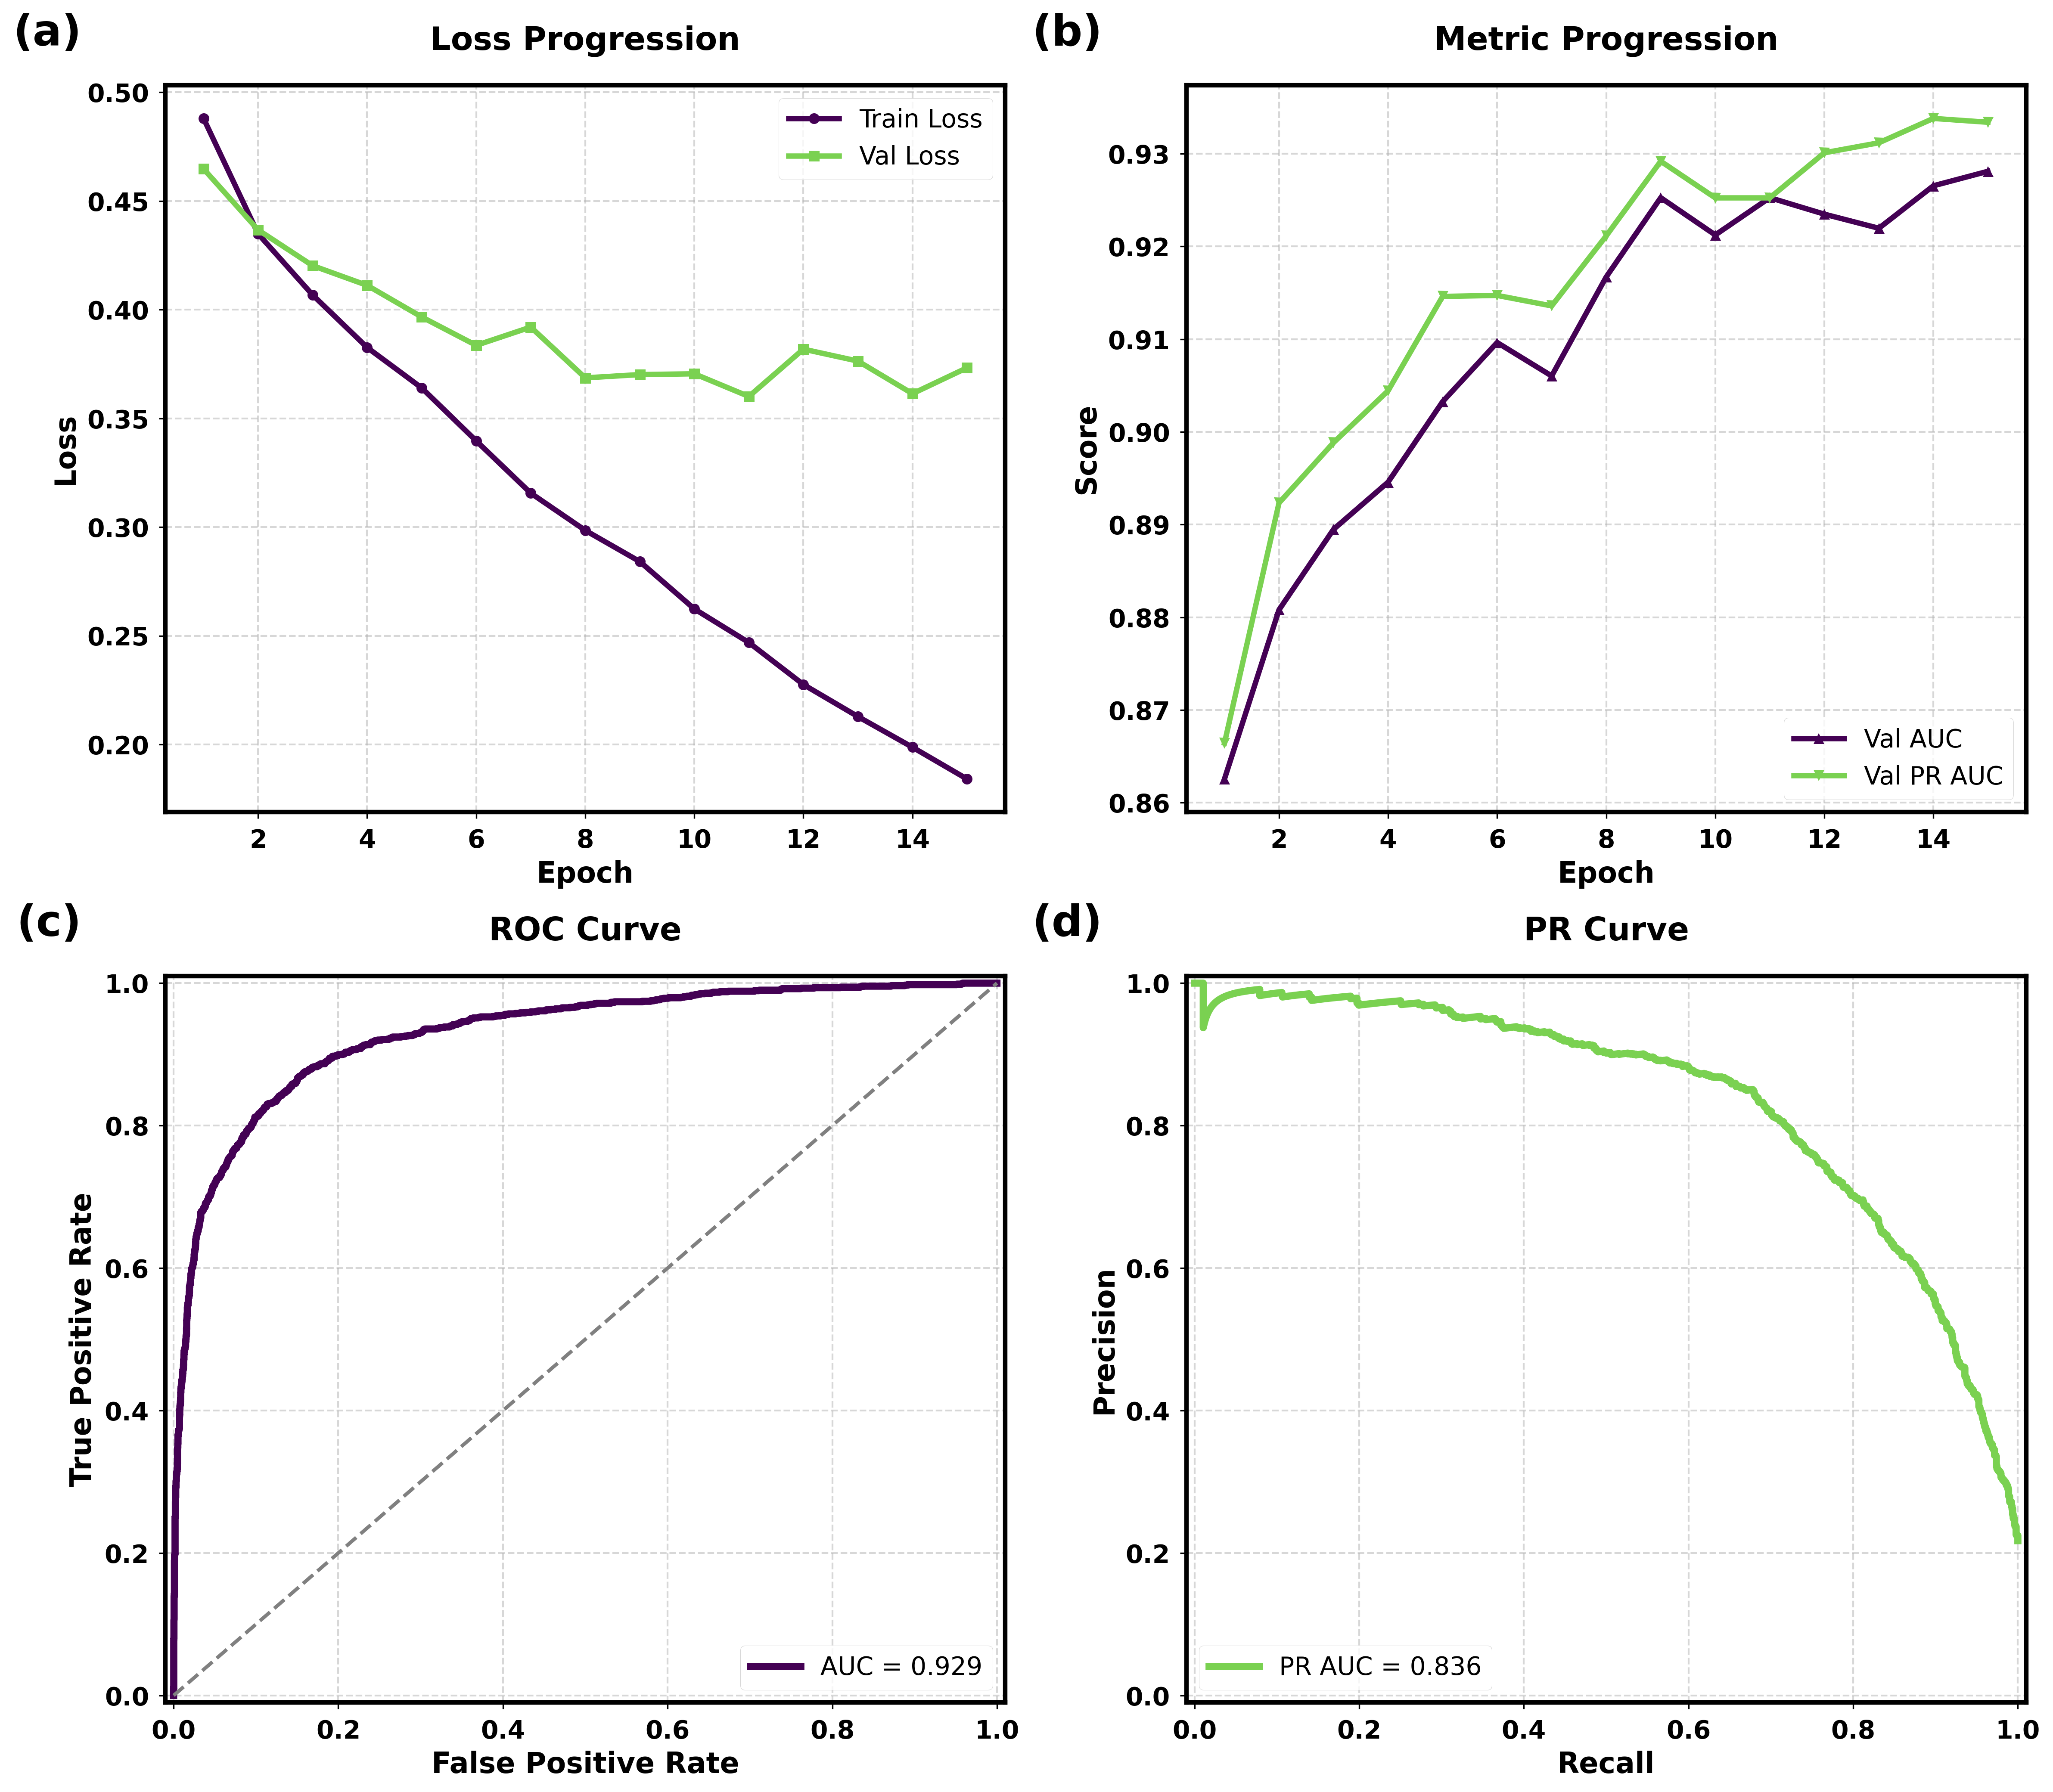
\includegraphics[width=1\textwidth]{figures/Fig2.png}
    \caption[模型训练过程与性能评估结果]{模型训练过程与性能评估结果。(a) 训练集与验证集损失；(b) 验证集 AUROC 与 PR-AUC；(c) 独立测试集 ROC 曲线；(d) 独立测试集 PR 曲线。}
    \label{fig:training_curves}
\end{figure}

如图~\ref{fig:training_curves}(a) 所示，训练损失在整个训练阶段持续下降，由初始阶段的 0.48 降至第 15 个 epoch 的 0.18，表明模型参数在不断逼近经验风险最小化解。与此同时，验证损失在前期快速下降，并在第 10 个 epoch 之后逐渐趋于稳定，在第 15 个 epoch 达到最低值 0.3732，未出现显著回升现象。这一现象说明模型在训练过程中未发生明显过拟合。

图~\ref{fig:training_curves}(b) 进一步表明，验证集 AUROC 从首个 epoch 的 0.8626 快速提升至第 15 个 epoch 的 0.9281，PR-AUC 同步提高至 0.9334，后期提升幅度显著减小并逐步进入平台期。该现象说明模型已充分学习到蛋白序列嵌入中蕴含的进化约束与功能语义信息，泛化性能趋于收敛。

在监督学习框架下，训练目标本质上是最小化训练集损失，因此训练误差持续下降是正常现象。然而，模型性能的关键评判标准并非训练误差，而是验证集上的泛化能力。随着训练轮次增加，模型可能逐渐开始拟合训练数据中的细微噪声，从而对泛化性能贡献有限。基于验证集损失与性能指标的综合考量，早停策略在第 15 个 epoch 终止训练，并选取验证集性能最优的模型参数用于后续测试。

从统计学习理论角度来看，当前训练过程呈现“训练误差持续降低、验证误差趋于稳定、泛化间隙保持可控”的特征，说明模型复杂度与样本规模之间达成了较为合理的平衡。在偏差–方差权衡框架下，模型已进入低偏差区域，而未观察到显著方差膨胀迹象，因此无需进一步延长训练周期。

为进一步评估模型的泛化能力，本研究选取验证集性能最优的模型参数，并在独立测试集上进行系统评估。测试集性能指标如表~\ref{tab:test_metrics} 所示：
在必需蛋白仅占约 22\% 的类别不平衡条件下，模型仍取得 0.8245 的 AUPRC 与 0.8187 的 Recall，表明其对少数类样本具有较高敏感性。Precision 为 0.6758，反映模型在保证召回率的同时维持了相对合理的误报控制能力。综合指标 F1-score 为 0.7404，说明模型在精准度与覆盖度之间取得了较为均衡的表现。

独立测试集的 ROC 曲线与 PR 曲线分别见图~\ref{fig:training_curves}(c) 与 (d)，
AUC 分别达到 0.9272 与 0.8245，表明模型具有较强判别能力。相较于验证集 AUROC（0.9281），测试集性能无差别，说明模型泛化稳定。

\begin{table}[!b]
\centering
\caption{模型在独立测试集上的性能指标}
\label{tab:test_metrics}
\begin{tabular}{lcccc}
\toprule
指标 & Accuracy & Recall & Precision & F1-score \\
\midrule
评估值 & 0.8752 & 0.8187 & 0.6758 & 0.7404 \\
\bottomrule
\end{tabular}
\end{table}

整体而言，模型在独立测试集上表现出稳定且可泛化的判别能力，为后续免疫相关依赖模型构建与中性粒细胞特异依赖蛋白筛选提供了可靠的算法基础。

本章完成了基于 ProtT5 嵌入与单头注意力机制的必需性预测模型构建。独立测试集上的 AUROC 与 AUPRC 指标验证了模型在高维语义表示空间中的判别能力与稳健性。下一章将进一步利用模型输出的 PES，对免疫情境中的蛋白功能依赖关系进行系统分群与特征解析。
